
\begin{frame}[t]{Áurea}
	O método de localização de mínimo da seção áurea é um aprimoramento do método de Fibonacci e faz uso da razão áurea,
	
	\begin{equation}
		R = \dfrac{\sqrt{5}-1}{2} \simeq 0.618
	\end{equation}
	
	\begin{figure}[h]
		\begin{center}
			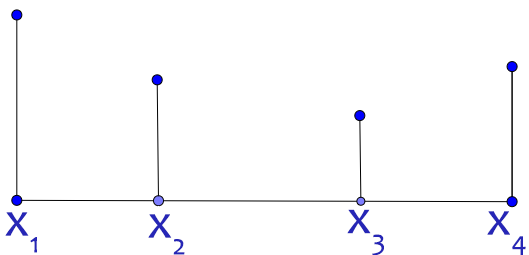
\includegraphics[width=6cm]{./aurea_ex.png}   
			\caption{Algoritmo de seção áurea}
			\label{fig:aurea_ex}
		\end{center}
	\end{figure}
\end{frame}